\cleardoublepage

\chapter{Arquitectura}
\label{makereference4}

\section{Equipamiento}
\label{makereference4.1}

Existen múltiples niveles de implementación del prototipo planteado en este documento. En función de la cantidad de módulos operativos se requerirá una mayor cantidad de hardware para la sensorización y los actuadores implicados. El nivel más básico e imprescindible implica un ordenador con SO Linux que actuara como controlador de la infraestructura de dispositivos que dan forma al sistema en su conjunto, esto es el Nodo.

\section{Definición del nodo principal}
\label{makereference4.2}

El \gls{gateway} representa el núcleo de una suite domótica. Los sensores y actuadores dispuestos en un hogar lo usan como centro neurálgico para que el sistema opere. Si bien los sensores son capaces de registrar datos por su cuenta, estos deben ser entregados en el \gls{gateway} para ser útiles. 

Como soporte de hardware  se usara un ordenador compacto de la marca Raspberry Pi. La selección particular de este dispositivo se apoya en dos características esenciales en el desarrollo de este proyecto: es barato, de bajo consumo eléctrico y su licenciamiento es libre. Además, goza de presencia en el mercado de electrónica, por lo cual es fácil de adquirir y ha acumulado una extensa comunidad de usuarios que muestran su uso mediante tutoriales y experimentos. Como motivos adicionales se encuentra su reducido tamaño que permite ubicarlo con facilidad en lugares estrechos o difícilmente accesibles y su imperceptible ruido al operar. El modelo concreto para el desarrollo del prototipo es Rapsberry Pi3b+ que dispone de capacidad de procesador y memoria RAM suficiente para operar todo el software necesario. Este modelo no integra un almacenamiento interno para el usuario, pero su interfaz incluye una ranura de tarjetas micro-SD compatible con todas las opciones de tamaño de almacenamiento disponibles en el mercado. Se precisan de al menos 4 \gls{gb} de espacio disponible en la memoria del sistema, y es recomendable exceder este mínimo siempre que sea posible, ya que la acumulación de datos con el paso del tiempo por parte del dispositivo crecerá indefinidamente.

\begin{figure}[hbt!]
\centering
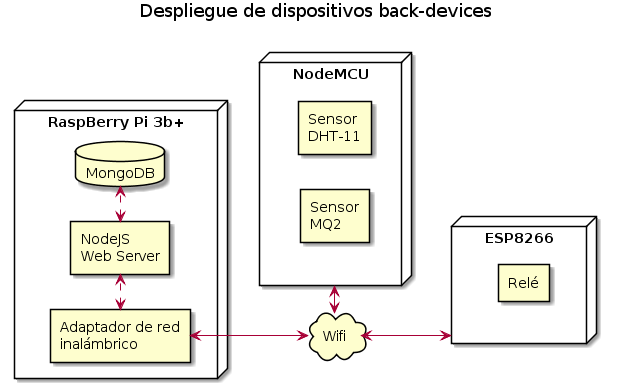
\includegraphics[height=2.5in]{figures/diagrams/physical-devices/back-devices.png}
\caption[Diagrama de despliegue de back-end]{Diagrama de despliegue de dispositivos y gateway\footnotemark}
\end{figure}

\section{Criterio de selección del dispositivos y Software}
\label{makereference4.3}

\begin{figure}[hbt!]
\centering
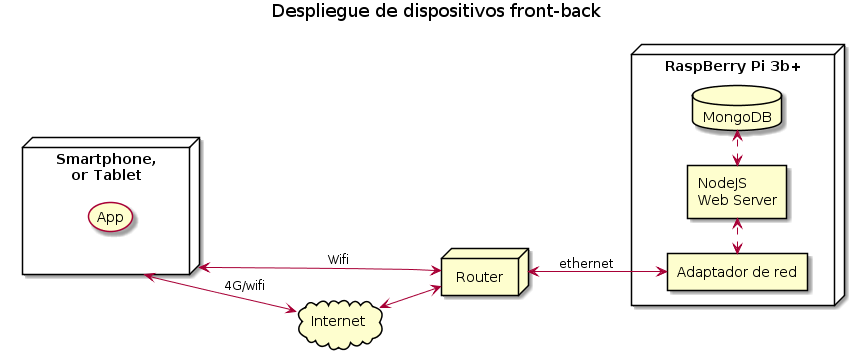
\includegraphics[height=2.5in]{figures/diagrams/physical-devices/front-back.png}
\caption[Despligue de front]{despliegue de front\footnotemark}
\end{figure}

\section{Criterio de selección servicios}
\label{makereference4.4}
La selección de un servicio para la gestión de la \gls{bbdd}


Podría parecer que hablamos de una relación de objetos entre sí, y que un modelo de \gls{bbdd} relacional es la mejor opción, pero si consideramos que, cada entrada almacenada tendrá una estructura distinta, hace que no sea una opción tan ideal. Pensemos, por ejemplo, que utilizando una \gls{bbdd} SQL se planifica un conjunto de tablas relacionadas entre sí. Sera necesaria una tabla que contenga las ubicaciones y se relacione con otra tabla que definan a los dispositivos. Esto establece una relación 1:N donde múltiples dispositivos pueden existir para una estancia, pero nunca en varias a la vez. De cada dispositivo existirá una nueva relación 1:N de medidas. Lo cual deja un esquema semejante al de la figura siguiente:


\begin{figure}[hbt!]
\centering
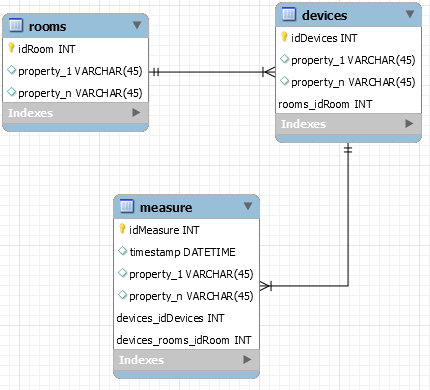
\includegraphics[height=2.5in]{figures/SQLSchemaExample_1.png}
\caption[Primer planteamiento de diseño de BBDD relacional]{Primer planteamiento de diseño de BBDD relacional\footnotemark}
\end{figure}

\vspace{1.5cm}

Sin embargo, existen algunos problemas graves de diseño de esta idea, en primer lugar, los dispositivos no pueden ser una propiedad de una estancia. Son objetos relacionados, pero no existe una transitividad dura entre ellos. Un dispositivo puede cambiar de estancia en un momento dado, y aun asi, seguir existiendo medidas en fechas concretas de ese dispositivo para una habitación en la cual, dicho dispositivo ya no está relacionado. Otro posible escenario es la desaparición de una estancia (como resultado de fusionar 2 estancias en una al derribar una pared). Para mantener una integridad lógica y persistente a lo largo del tiempo. Toda medida deberá tener un campo que determine en que ubicación fue tomada.
no hay transitividad dura entre room y device, lo cual hace que sean independientes entre sí.


\begin{figure}[hbt!]
\centering
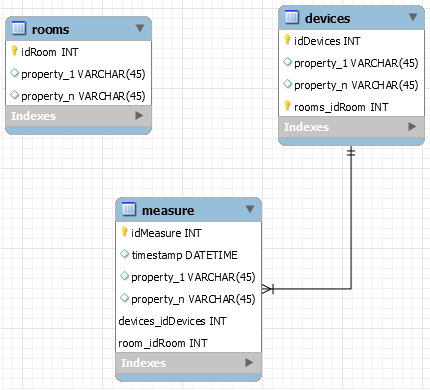
\includegraphics[height=2.5in]{figures/SQLSchemaExample_2.png}
\caption[Segundo planteamiento de diseño de BBDD relacional]{Primer planteamiento de diseño de BBDD relacional\footnotemark}
\end{figure}

\vspace{1.5cm}

Con esto aún tendríamos que enfrentar un problema adicional, el número de columnas que definen las propiedades de una tabla. El ejemplo más claro es la tabla de medidas. Una medida, efectuada por un sensor será definida por su identificador y la fecha en la que se realizó, ahora bien, según la naturaleza del dispositivo, se obtendrán disantos tiempos de medida. Un sensor combinado de temperatura y humedad nos dará dos magnitudes de medición, un sensor de ruido almacenará un valor de decibelios, una luz define su medida por su estado de actividad (encendido o apagado), aunque por otra parte podría indicar el consumo eléctrico, o propiedades adicionales como intensidad de luz, o incluso color. Es cierto que, para un actuador, como lo es un emisor de luz, no realiza medidas como tal, y sus correspondientes estados de actividad podrían ser más adecuados definirlos como propiedades del dispositivo y no como medidas. Podríamos separar las medidas de los estados en tablas distintas, pero igualmente llegaríamos al problema del número de campos necesarios en una tabla. Valor que por otra parte es muy difícil de prever en base a la extensa gama de dispositivos existentes. Esto puede solucionarse de manera sencilla con 2 estrategias. Incluir una gran cantidad de columnas en previsión de los distritos tipos de medidas existentes, dejando que las medidas posean un valor nulo para los campos no utilizados en función de la relación de su sensor, o bien, unificar todos los campos en un único valor de cadena de caracteres que almacene un dato estructurado, como es el caso de los JSON. Esta última opción, sería la más deseable tanto por sencillez de implementación como facilidad de procesamiento. Lo que dejaría un esquema semejante a este:

\begin{figure}[hbt!]
\centering
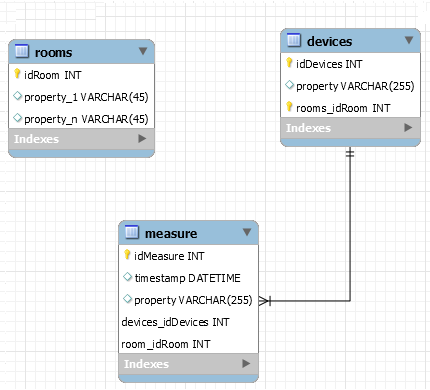
\includegraphics[height=2.5in]{figures/SQLSchemaExample_3.png}
\caption[Tercer planteamiento de diseño de BBDD relacional]{Primer planteamiento de diseño de BBDD relacional\footnotemark}
\end{figure}

Una preocupación que agrava la perspectiva de usar una \gls{bbdd} relacional es, en este punto del proyecto, su escalabilidad horizontal. Si bien las tablas pueden crecer a un gran número de registros, no se prevé almacenar datos con vistas a largo plazo, la mayoría de los valores almacenados serán efímeros en tiempo de utilidad, almacenarlos responde solo a la necesidad de obtener comparativas en plazos de tiempo relativamente cortos, como horas, días, y posiblemente semanas. Mas allá de este rango estos datos no tienen una utilidad real y pueden ser condensados en medidas para utilizarse en resúmenes. Por otro lado, disponer de flexibilidad a la hora de configurar la extensión de propiedades de un objeto de la \gls{bbdd} es uno de los puntos fuertes de una \gls{bbdd} no relacional.
